\documentclass[a4paper,12pt]{article}
\usepackage[a4paper,landscape,margin=2cm]{geometry} % <-- orientamento orizzontale
\usepackage{tikz}
\usetikzlibrary{arrows.meta, positioning}

\title{Server Musei via openAPI (CRUD + REST)}
\author{Strutture del codice}
\date{\today}

\begin{document}

\maketitle

\section*{1. Panoramica delle strutture principali}

\begin{itemize}
  \item \textbf{Server HTTPS (openAPI\_server.js)}: punto di ingresso del sistema, gestisce le richieste HTTP.
  \item \textbf{SistemaMusei (sistema\_musei.js)}: struttura che contiene tutti i musei.
  \item \textbf{Museo (museo.js)}: rappresenta un singolo museo e gestisce i suoi oggetti.
  \item \textbf{Graph (graph.js)}: struttura a grafo per la connessione tra oggetti all'interno di un museo.
  \item \textbf{MongoDB (mongo\_upload.js)}: persistenza dei dati, sincronizza musei e oggetti su database.
  \item \textbf{parser\_musei.js}: carica musei da file JSON iniziale.
\end{itemize}

\section*{2. Connessioni tra le strutture}

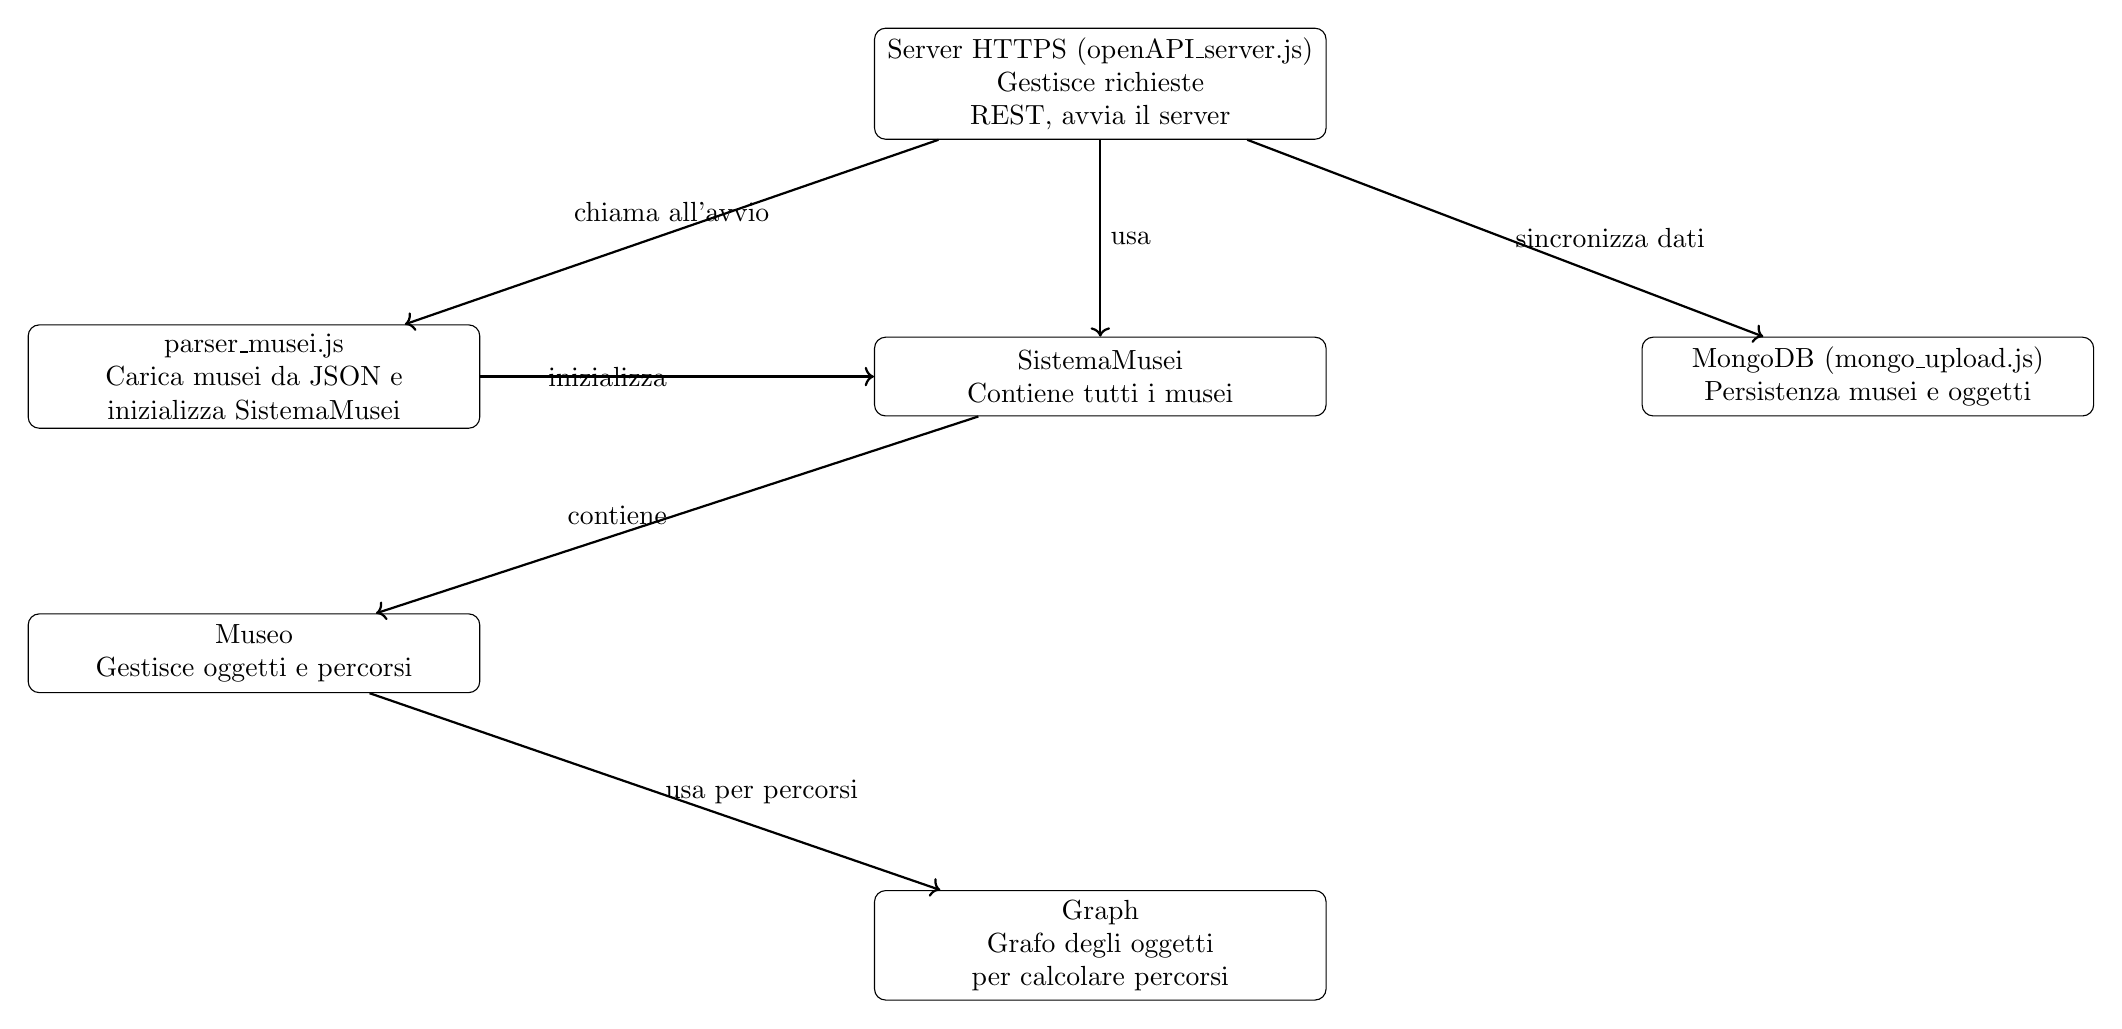
\begin{tikzpicture}[
  node distance=2.5cm and 5cm,
  box/.style={rectangle, draw, rounded corners, text width=5.5cm, align=center, minimum height=1cm}
]

\node[box] (server) {Server HTTPS (openAPI\_server.js)\\Gestisce richieste REST, avvia il server};
\node[box, below=of server] (sistema) {SistemaMusei\\Contiene tutti i musei};
\node[box, below left=of sistema] (museo) {Museo\\Gestisce oggetti e percorsi};
\node[box, below right=of museo] (graph) {Graph\\Grafo degli oggetti per calcolare percorsi};
\node[box, right=of sistema, xshift=-1cm] (mongo) {MongoDB (mongo\_upload.js)\\Persistenza musei e oggetti};
\node[box, left=of sistema] (parser) {parser\_musei.js\\Carica musei da JSON e inizializza SistemaMusei};

% Connessioni
\draw[->, thick] (server) -- (sistema) node[midway,right]{usa};
\draw[->, thick] (sistema) -- (museo) node[midway,left]{contiene};
\draw[->, thick] (museo) -- (graph) node[midway,right]{usa per percorsi};
\draw[->, thick] (server) -- (mongo) node[midway,right]{sincronizza dati};
\draw[->, thick] (parser) -- (sistema) node[midway,left]{inizializza};
\draw[->, thick] (server) -- (parser) node[midway,above]{chiama all'avvio};

\end{tikzpicture}

\pagebreak
\section*{3. Funzionamento ad alto livello}

\begin{enumerate}
  \item Il \textbf{server HTTPS} riceve richieste API.
  \item Viene usato \textbf{SistemaMusei} per ottenere o modificare dati dei musei.
  \item Ogni \textbf{Museo} gestisce i suoi \textbf{oggetti} e usa il \textbf{Graph} per calcolare percorsi tra oggetti.
  \item Tutte le modifiche vengono salvate su file JSON e sincronizzate con \textbf{MongoDB}.
  \item All'avvio, \textbf{parser\_musei.js} carica il JSON e inizializza \textbf{SistemaMusei}.
\end{enumerate}

\section*{4. Note aggiuntive}
\begin{itemize}
  \item Middleware sicurezza gestisce API key e CORS.
  \item Logging delle richieste per debug.
  \item HTTPS con certificati TLS, opzionale solo localhost.
\end{itemize}

\section*{5. Sicurezza e protezione}

\begin{itemize}
  \item \textbf{API Key}: tutte le richieste devono includere un header \texttt{x-api-key} valido per essere autorizzate.
  \item \textbf{Connessione limitata a localhost}: il server accetta richieste solo da \texttt{localhost} (127.0.0.1).
  \item \textbf{TLS / HTTPS}: tutte le comunicazioni avvengono tramite HTTPS per garantire cifratura dei dati in transito.
  \item \textbf{Autenticazione}: il server verifica la chiave API prima di processare qualsiasi richiesta REST.
  \item \textbf{Uso tipico}: in sviluppo, i certificati TLS possono essere self-signed; in produzione sarebbe necessario un certificato valido.
\end{itemize}


\end{document}

